% Template of basic phisics experiment 基于 article template, 在此基础上做修改
% 设定文章编码类型, 正文字号为五号则 zihao=5, 正文字号为小四则 zihao=-4
\documentclass[zihao=5, UTF8]{article}


% 自定义宏定义
\def\N{\mathbb{N}}
\def\F{\mathbb{F}}
\def\Z{\mathbb{Z}}
\def\Q{\mathbb{Q}}
\def\R{\mathbb{R}}
\def\C{\mathbb{C}}
\def\T{\mathbb{T}}
\def\S{\mathbb{S}}
\def\A{\mathbb{A}}
\def\I{\mathscr{I}}
\def\d{\mathrm{d}}
\def\p{\partial}


% 物理实验报告所需的其它宏包
\usepackage{ulem}   % \uline 下划线支持

% 导入基本宏包
\usepackage[UTF8]{ctex}     % 设置文档为中文语言
\usepackage[colorlinks, linkcolor=blue, anchorcolor=blue, citecolor=blue, urlcolor=blue]{hyperref}  % 宏包: 自动生成超链接 (此宏包与标题中的数学环境冲突)
% \usepackage{docmute}    % 宏包: 子文件导入时自动去除导言区, 用于主/子文件的写作方式, \include{./51单片机笔记}即可. 注: 启用此宏包会导致.tex文件capacity受限.
\usepackage{amsmath}    % 宏包: 数学公式
\usepackage{physics}
\usepackage{bm}
\usepackage{mathrsfs}   % 宏包: 提供更多数学符号
\usepackage{amssymb}    % 宏包: 提供更多数学符号
\usepackage{pifont}     % 宏包: 提供了特殊符号和字体
\usepackage{extarrows}  % 宏包: 更多箭头符号
\usepackage{multirow}
\usepackage{siunitx}

\renewcommand{\dd}{\mathrm{d}}

% 列表环境设置
\usepackage{enumitem}   % 宏包: 列表环境设置
    \setlist[enumerate]{itemsep=0pt, parsep=0pt, topsep=0pt, partopsep=0pt, leftmargin=3.5em}
    \setlist[itemize]{itemsep=0pt, parsep=0pt, topsep=0pt, partopsep=0pt, leftmargin=3.5em}
    \newlist{circledenum}{enumerate}{1} % 创建一个新的枚举环境
    \setlist[circledenum,1]{
        label=\protect\circled{\arabic*}, % 使用 \arabic* 来获取当前枚举计数器的值, 并用 \circled 包装它
        ref=\arabic*, % 如果需要引用列表项, 这将决定引用格式(这里仍然使用数字)
        itemsep=0pt, parsep=0pt, topsep=0pt, partopsep=0pt, leftmargin=3.5em
    }
% 文章页面 margin 设置
\usepackage[a4paper]{geometry}  % 宏包: 文章页面 margin 设置
    \geometry{top=0.75in}
    \geometry{bottom=0.75in}
    \geometry{left=0.75in}
    \geometry{right=0.75in}   % 设置上下左右页边距
    \geometry{marginparwidth=1.75cm}    % 设置边注距离(注释、标记等)

% 自定义数学环境
\usepackage{amsthm} % 宏包: 数学环境配置
% theorem-line 环境自定义
    \newtheoremstyle{MyLineTheoremStyle}% <name>
        {11pt}% <space above>
        {11pt}% <space below>
        {}% <body font> 使用默认正文字体
        {}% <indent amount>
        {\bfseries}% <theorem head font> 设置标题项为加粗
        {: }% <punctuation after theorem head>
        {.5em}% <space after theorem head>
        {\textbf{#1}\thmnumber{#2}\ \ (\,\textbf{#3}\,)}% 设置标题内容顺序
    \theoremstyle{MyLineTheoremStyle} % 应用自定义的定理样式
    \newtheorem{LineTheorem}{Theorem.\,}
% theorem-block 环境自定义
    \newtheoremstyle{MyBlockTheoremStyle}% <name>
        {11pt}% <space above>
        {11pt}% <space below>
        {}% <body font> 使用默认正文字体
        {}% <indent amount>
        {\bfseries}% <theorem head font> 设置标题项为加粗
        {: \\ \indent}% <punctuation after theorem head>
        {.5em}% <space after theorem head>
        {\textbf{#1}\thmnumber{#2}\ \ (\,\textbf{#3}\,)}% 设置标题内容顺序
    \theoremstyle{MyBlockTheoremStyle} % 应用自定义的定理样式
    \newtheorem{BlockTheorem}[LineTheorem]{Theorem.\,} % 使用 LineTheorem 的计数器
% definition 环境自定义
    \newtheoremstyle{MySubsubsectionStyle}% <name>
        {11pt}% <space above>
        {11pt}% <space below>
        {}% <body font> 使用默认正文字体
        {}% <indent amount>
        {\bfseries}% <theorem head font> 设置标题项为加粗
        {: \\ \indent}% <punctuation after theorem head>
        {0pt}% <space after theorem head>
        {\textbf{#3}}% 设置标题内容顺序
    \theoremstyle{MySubsubsectionStyle} % 应用自定义的定理样式
    \newtheorem{definition}{}


% 有色文本框及其设置
\usepackage[dvipsnames,svgnames]{xcolor}    %设置插入的文本框颜色
\usepackage[strict]{changepage}     % 提供一个 adjustwidth 环境
\usepackage{framed}     % 实现方框效果
    \definecolor{graybox_color}{rgb}{0.95,0.95,0.96} % 文本框颜色. 修改此行中的 rgb 数值即可改变方框纹颜色, 具体颜色的rgb数值可以在网站https://colordrop.io/ 中获得. (截止目前的尝试还没有成功过, 感觉单位不一样)(找到喜欢的颜色, 点击下方的小眼睛, 找到rgb值, 复制修改即可)
    \newenvironment{graybox}{%
    \def\FrameCommand{%
    \hspace{1pt}%
    {\color{gray}\small \vrule width 2pt}%
    {\color{graybox_color}\vrule width 4pt}%
    \colorbox{graybox_color}%
    }%
    \MakeFramed{\advance\hsize-\width\FrameRestore}%
    \noindent\hspace{-4.55pt}% disable indenting first paragraph
    \begin{adjustwidth}{}{7pt}%
    \vspace{2pt}\vspace{2pt}%
    }
    {%
    \vspace{2pt}\end{adjustwidth}\endMakeFramed%
    }

% 各级标题自定义设置
\usepackage{titlesec}
    % section标题自定义设置
    \titleformat{\section}[hang]{\normalfont\huge\bfseries\centering}{第\,\thesection\,部分}{20pt}{}
    % subsection标题自定义设置
    \titleformat{\subsection}[hang]{\normalfont\Large\bfseries}{\,\thesubsection\,}{8pt}{}
    % subsubsection标题自定义设置
    \titleformat{\subsubsection}[hang]{\normalfont\large\bfseries}{\,\thesubsubsection\,}{6pt}{}

% 外源代码插入设置
\usepackage{matlab-prettifier}
    \lstset{
        style=Matlab-editor,  % 继承matlab代码颜色等
    }
\usepackage[most]{tcolorbox} % 引入tcolorbox包
\usepackage{listings} % 引入listings包
    \tcbuselibrary{listings, skins, breakable}
    \lstdefinestyle{matlabstyle}{
        language=Matlab,
        basicstyle=\small,
        breakatwhitespace=false,
        breaklines=true,
        captionpos=b,
        keepspaces=true,
        numbers=left,
        numbersep=15pt,
        showspaces=false,
        showstringspaces=false,
        showtabs=false,
        tabsize=2
    }
    \newtcblisting{matlablisting}{
        arc=0pt,
        top=0pt,
        bottom=0pt,
        left=1mm,
        listing only,
        listing style=matlabstyle,
        breakable,
        colback=white   % 选一个合适的颜色
    }

% table 支持
\usepackage{booktabs}   % 宏包: 三线表
\usepackage{tabularray} % 宏包: 表格排版
\usepackage{longtable}  % 宏包: 长表格

% figure 设置
\usepackage{graphicx}  % 支持 jpg, png, eps, pdf 图片
\usepackage{svg}       % 支持 svg 图片
    \svgsetup{
        % 指向 inkscape.exe 的路径
        inkscapeexe = C:/aa_MySame/inkscape/bin/inkscape.exe,
        % 一定程度上修复导入后图片文字溢出几何图形的问题
        inkscapelatex = false
    }


% 图表进阶设置
\usepackage{float}     % 图表位置浮动设置
\usepackage{caption}    % 图注、表注
    \captionsetup[figure]{name=图}
    \captionsetup[table]{name=表}
    \captionsetup{labelfont=bf, font=small}

%% 文章默认字体设置
%    \usepackage{fontspec}   % 宏包: 字体设置
%        \setmainfont{SimSun}[
%            BoldFont = SimHei, % 设置粗体字为黑体
%            ItalicFont = KaiTi, % 设置斜体字为楷体
%            BoldItalicFont = KaiTi % 设置粗斜体字为楷体
%        ]
%        %\setCJKmainfont[AutoFakeBold=3]{SimSun} % 设置加粗字体为 SimSun 族, AutoFakeBold 可以调整字体粗细
%        \setmainfont{Times New Roman} % 设置英文字体为Times New Roman


% 其它设置
    % equation 公式编号设置
        \makeatletter
        \renewcommand{\theequation}{\thesection.\arabic{equation}}
        \makeatother
    % 脚注设置
        \renewcommand\thefootnote{\ding{\numexpr171+\value{footnote}}}
    % 参考文献引用设置
        \bibliographystyle{unsrt}   % 设置参考文献引用格式为unsrt
        \newcommand{\upcite}[1]{\textsuperscript{\cite{#1}}}     % 自定义上角标式引用
    % 文章序言设置
        \newcommand{\cnabstractname}{序言}
        \newenvironment{cnabstract}{%
            \par\Large
            \noindent\mbox{}\hfill{\bfseries \cnabstractname}\hfill\mbox{}\par
            \vskip 2.5ex
            }{\par\vskip 2.5ex}


% 页眉页脚设置
\usepackage{fancyhdr}   %宏包: 页眉页脚设置
    \pagestyle{fancy}
    \fancyhf{}
    \cfoot{\thepage}
    \renewcommand\headrulewidth{1pt}
    \renewcommand\footrulewidth{0pt}
    \rhead{\bfseries 分组序号: 3-04-1}
    \chead{《基础物理实验》实验报告,\ 潘天麟\ 2023K8009908023}
    \lhead{2024.12.11}

\usepackage{pdfpages}

% 开始编辑文章

\begin{document}
\noindent\begin{flushright}
    \zihao{2}{分组序号: 3-04-1}
\end{flushright}

\newcommand*{\boldsong}{\CJKfamily{boldsong}}


\begin{center}\large
    \noindent{\Huge\bfseries\boldsong《基础物理实验》实验报告 }
    \\\vspace{0.4cm}
    \noindent\textit{
        \textbf{\boldsong 实验名称: }\uline{\hspace{2.3cm} 虚拟仪器\hspace{2.3cm}}\hspace{0.4cm}
        指导教师: \uline{\hspace{1.5cm} 暴子瑜 \hspace{1.5cm}}}
    \\\vspace{0.1cm}
    \noindent\textit{
        姓名: \uline{\,\,潘天麟\,\,}\hspace{0.2cm}
        学号: \uline{\,\,{\upshape 2023K8009908023}\,\,}\hspace{0.2cm}
        专业: \uline{\,\,人工智能\,\,}\hspace{0.2cm}
        班级: \uline{\,\,\upshape{2313}\,\,}\,组号: \uline{\,\,\upshape{3-04-1}\,\,}}
    \\\vspace{0.1cm}
    \noindent\textit{
        实验日期: \uline{\,\,{\upshape 2024.12.11}\,\,}\hspace{0.2cm}
        实验地点: \uline{\,\,\,教学楼{\upshape 702}\,\,\,}\hspace{0.2cm}
        是否调课/补课: \uline{\,\,否\,\,}\hspace{0.2cm}
        成绩: \uline{\hspace{2cm}}}
\end{center}
% \vspace{-0.2cm}
\noindent\rule{\textwidth}{0.1em}   % 分割线

% 控制目录不换页
\vspace{1cm}
\setcounter{tocdepth}{3}  % 目录深度为 2(不显示 subsubsection)
\noindent\begin{minipage}{\textwidth}\centering
\tableofcontents\thispagestyle{fancy}   % 显示页码、页眉等
\end{minipage}
\newpage

\section{实验目的}
\begin{enumerate}
    \item 了解虚拟仪器的概念.
    \item 了解图形化编程语言LabVIEW, 学习简单的LabVIEW编程；
    \item 完成伏安法测电阻的虚拟仪器设计.
\end{enumerate}

\section{实验仪器}

\begin{itemize}
    \item 计算机
    \item LabVIEW 2014
    \item NI ELVIS II$^+$
    \item 导线若干
    \item 元件盒一个, 包括以下元件:
        \begin{itemize}
            \item 100\,$\Omega$ 标准电阻1个
            \item 待测电阻: 1\,k$\Omega$ 和 51\,$\Omega$ 各1个
            \item 稳压二极管1个
        \end{itemize}
    \item 热电偶等其他元件
\end{itemize}

\section{实验原理}

\subsection{虚拟仪器的硬件}
本实验使用的硬件平台是计算机, 结合了美国国家仪器公司 (National Instruments) 的教学实验室虚拟仪器套件II+ (缩写为 NI ELVIS II+) 和自带的原型板. 此套件允许用户通过计算机来控制实验设备, 并获取测量数据.

\subsection{虚拟仪器的软件}
本实验采用LabVIEW软件开发平台作为虚拟仪器的编程环境. LabVIEW是一种图形化编程语言, 它将计算机的数据分析和显示能力与仪器驱动程序整合在一起, 极大地简化了仪器编程的过程. 用LabVIEW开发的虚拟仪器程序称为VI (Virtual Instrument) , 每个VI由三个主要部分组成:
\begin{itemize}
    \item \textbf{前面板 (Front Panel) }: 用于设置输入数值和显示输出量, 相当于传统仪器的前面板.
    \item \textbf{程序框图 (Block Diagram) }: 实现仪器内部功能的逻辑结构, 包含端口、节点、图框和连线等元素.
    \item \textbf{图标/连线板 (Icon/Connector Pane) }: 用于定义VI的外观和接口.
\end{itemize}

\subsection{使用虚拟仪器测量伏安特性}
在本次实验中, 我们使用一个模拟输出通道为整个测量电路供电, 并利用两个模拟输入通道分别测量总电压与标准电阻上的电压, 如图\ref{fig:va_characteristic}所示.

\begin{figure}[H]
    \centering
    
\includegraphics[width=0.4\textwidth]{fig1.png}
    \caption{用虚拟仪器测量伏安特性原理图}
    \label{fig:va_characteristic}
\end{figure}

通过总电压和标准电阻上的电压值, 可以计算出总电流以及待测电阻上的电压. 通过程序设定, 从0V开始逐步增加总电压至设定值, 并在每次改变电压后记录相应的电流值, 最终得到一组电流-电压数据. 对这些数据进行线性拟合后, 即可获得待测电阻的阻值.

\section{实验内容}
\subsection{创建一个温度测量程序}
首先, 在电脑中打开LabVIEW 2014软件, 并新建一个VI. 在前面板中打开控件选板, 选择以下控件并加入到前面板中:
\begin{itemize}
    \item 温度计
    \item 垂直滑动杆开关 (条件真处标签为“华氏”, 条件假处标签为“摄氏”)
    \item 数值显示控件 (命名为“温度值”)
    \item 数值输入控件 (命名为“采集的电压”)
\end{itemize}
调整各控件位置, 如图\ref{fig:temperature_front_panel}所示.

\begin{figure}[H]
    \centering
    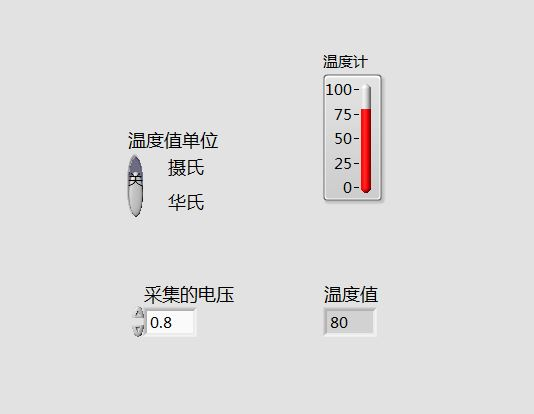
\includegraphics[width=0.4\textwidth]{data/exp1-fig1.JPG}
    \caption{温度测量程序前面板}
    \label{fig:temperature_front_panel}
\end{figure}

随后, 在程序框图中插入乘法函数、减法函数、除法函数以及选择函数, 按照讲义内容连接这些函数, 以实现所需的计算逻辑, 具体结果如图\ref{fig:temperature_block_diagram}所示.

\begin{figure}[H]
    \centering
    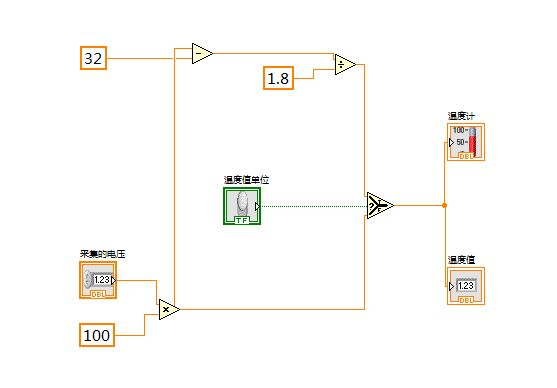
\includegraphics[width=0.8\textwidth]{data/exp1-fig2.JPG}
    \caption{温度测量程序程序框图}
    \label{fig:temperature_block_diagram}
\end{figure}

所有程序编写完成后, 在前面板中点击连续运行, 输入不同电压值并且切换温度单位, 观察温度变化是否符合预期.

\subsection{创建一个电压输出与采集程序}
新建一个VI, 在程序框图中建立虚拟输出通道, 设置为模拟输出电压. 右键点击该框图左上方出现的物理通道, 创建输入控件, 并选择“DAQmx开始任务”、“DAQmx写入”和“DAQmx清除任务”节点放入程序框图中. 在“DAQmx 写入”的图标数据输入端创建输入控件.

接着创建一个while循环, 放置定时器, 设置常量为100ms, 并在循环中添加停止输出按钮. 根据讲义整理图标和连线, 完成后的程序框图与前面板如图\ref{fig:voltage_io_block_diagram}和图\ref{fig:voltage_io_front_panel}所示.

\begin{figure}[h]
    \centering
    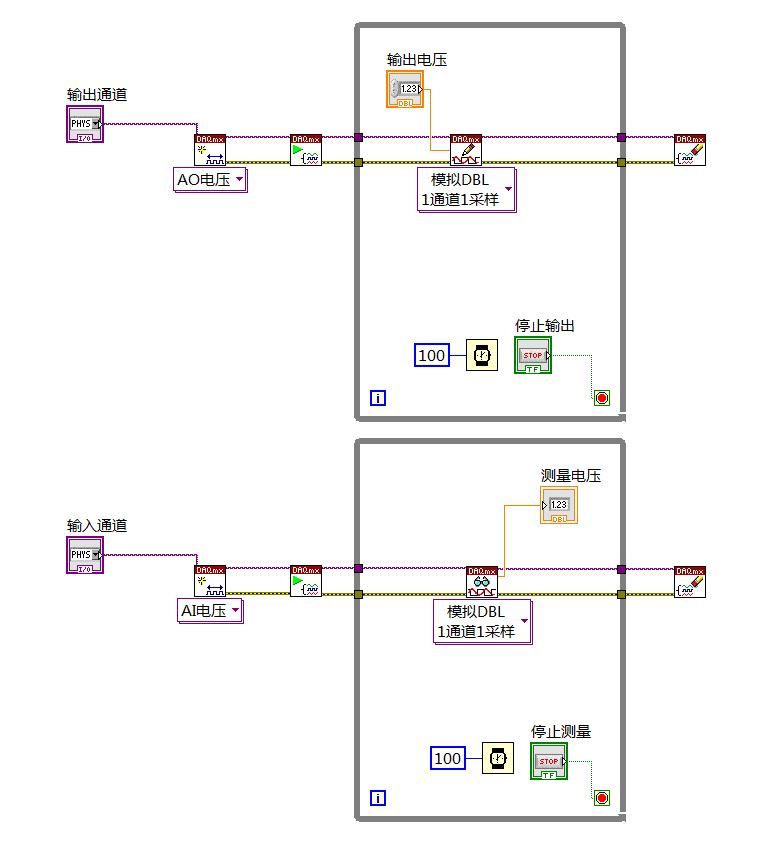
\includegraphics[width=0.8\textwidth]{data/exp2-fig2.JPG}
    \caption{电压采集与输出程序程序框图}
    \label{fig:voltage_io_block_diagram}
\end{figure}

\begin{figure}[h]
    \centering
    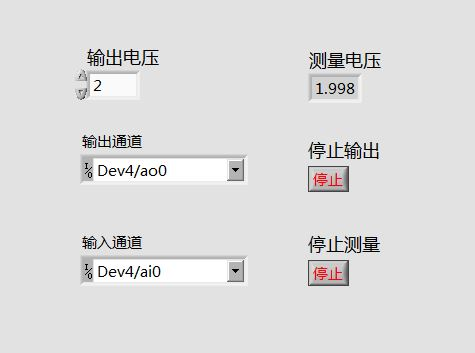
\includegraphics[width=0.6\textwidth]{data/exp2-fig1.JPG}
    \caption{电压采集与输出程序前面板}
    \label{fig:voltage_io_front_panel}
\end{figure}

设置前面板中的输出通道为Dev1/ao0, 输入通道为Dev1/ai0, 并在原型版上连接电路. 运行程序, 改变输入电压, 观察输出电压与输入电压是否一致.

\subsection{用虚拟仪器测量伏安特性曲线}
在前面板中放置一个Express XY图, 代表电流-电压图, 将其名称改为“电阻的伏安曲线图”, 并将横坐标命名为电压 (V) , 纵坐标命名为电流 (A) , 设置模式为“点-线”.

在前面板中插入四个数值型输入控件, 分别命名为“输出电压步长 (V) ”、“测量数据点数”、“标准电阻”、“时间间隔 (s) ”. 在“时间间隔”控件右方输入单位“s”, 同理在“输出电压步长”控件右方输入单位“V”. 再放入一个数值型显示控件, 命名为“待测电阻值”. 加入一个二维数组显示控件, 命名为“数据”, 用于显示测量的电压和电流. 放入一个开关按钮, 用于控制程序进程. 完成后的前面板如图\ref{fig:iv_curve_front_panel}所示.

\begin{figure}[H]
    \centering
    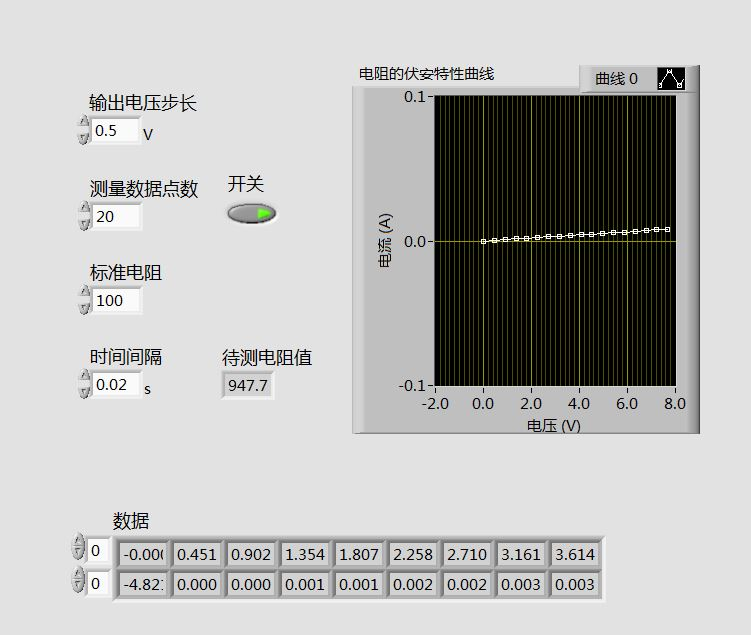
\includegraphics[width=0.6\textwidth]{data/exp3-fig1.JPG}
    \caption{伏安特性曲线程序前面板}
    \label{fig:iv_curve_front_panel}
\end{figure}

在程序框图中, 插入一个顺序结构, 添加5帧. 在各帧中按如下步骤操作:
\begin{enumerate}
    \item 第0帧: 放入一个DAQ助手, 选择“Dev1 (NI ELVIS II+) ”下的“ao 0”输出, 设置生成模式为“1采样 (按要求) ”.
    \item 第1帧: 放入一个等待节点, 并放入一个单位转换节点, 将单位转换为“ms”, 连接相关节点.
    \item 第2帧: 放入一个DAQ助手, 输入“Dev1 (NI ELVIS II+) ”下的“ai 0”和“ai 1”, 再放入两个索引数组, 连接DAQ中的数据输出端和数组中的数据端, 设置索引常量分别为0和1. 再放入“减”和“除”的节点.
    \item 第3帧: 放入一个“等待 (ms) ”节点, 设置常量数值为100ms.
    \item 第4帧: 放入一个“DAQ助手”, 使顺序结构结束时电压输出为0.
\end{enumerate}

在顺序结构外添加一个While循环, 比较While循环的i和“测量数据点数”控件中的值, 结合开关进行逻辑“与”运算, 控制循环. 添加移位寄存器存储并传递电压和电流的测量数据, 在循环中放入“创建数组”节点, 用于将新测量数据与原有数据组合成新的一维数组.

在程序框图中放入一个“创建数组”节点, 将电压和电流数据相连, 并将输出连接到名为“数据”的数组显示控件. 使用“创建XY图”显示伏安曲线, 连接电压数组和电流数组作为X和Y输入.

在循环外面放入一个“线性拟合”节点, 将电流数组和电压数组连接到“线性拟合”的X和Y输入端, 将“斜率”输出端连接到“待测电阻值”显示控件, 以显示电阻值. 整理前面板上的各图标位置, 并检查和整理程序框图中的连线. 最终结果如图\ref{fig:iv_curve_block_diagram}所示.

\begin{figure}[H]
    \centering
    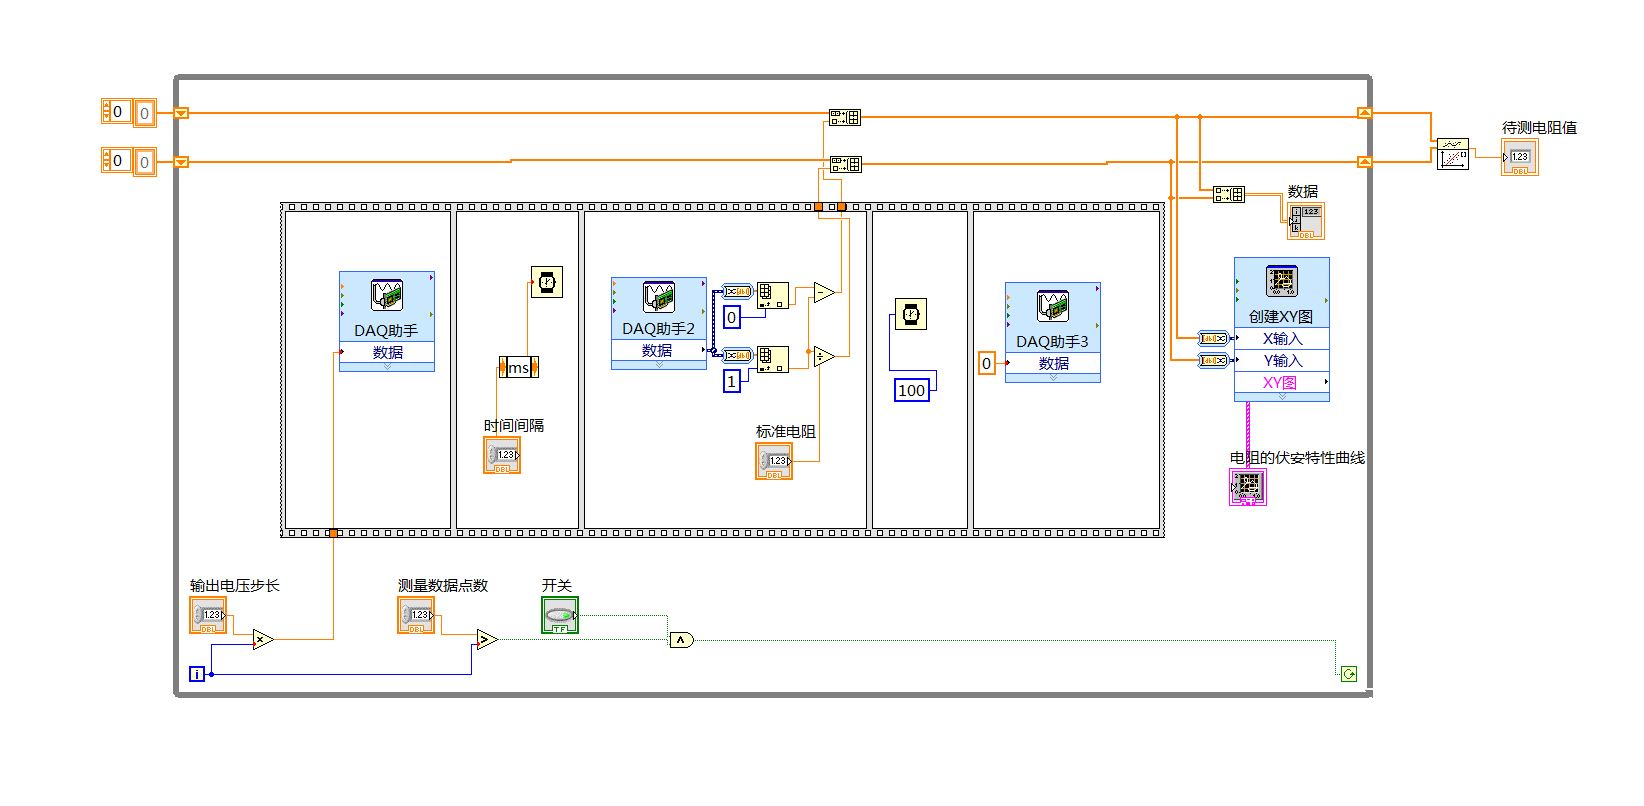
\includegraphics[width=1.0\textwidth]{data/exp3-fig2.JPG}
    \caption{伏安特性曲线程序程序框图}
    \label{fig:iv_curve_block_diagram}
\end{figure}

在原型版上正确连接电路如图, 运行后对不同电阻以及发光二极管进行测量, 获得一系列实验数据.
原型板的实际电路连接如图\ref{fig:iv_curve_circuit}所示.

\begin{figure}[H]
    \centering
    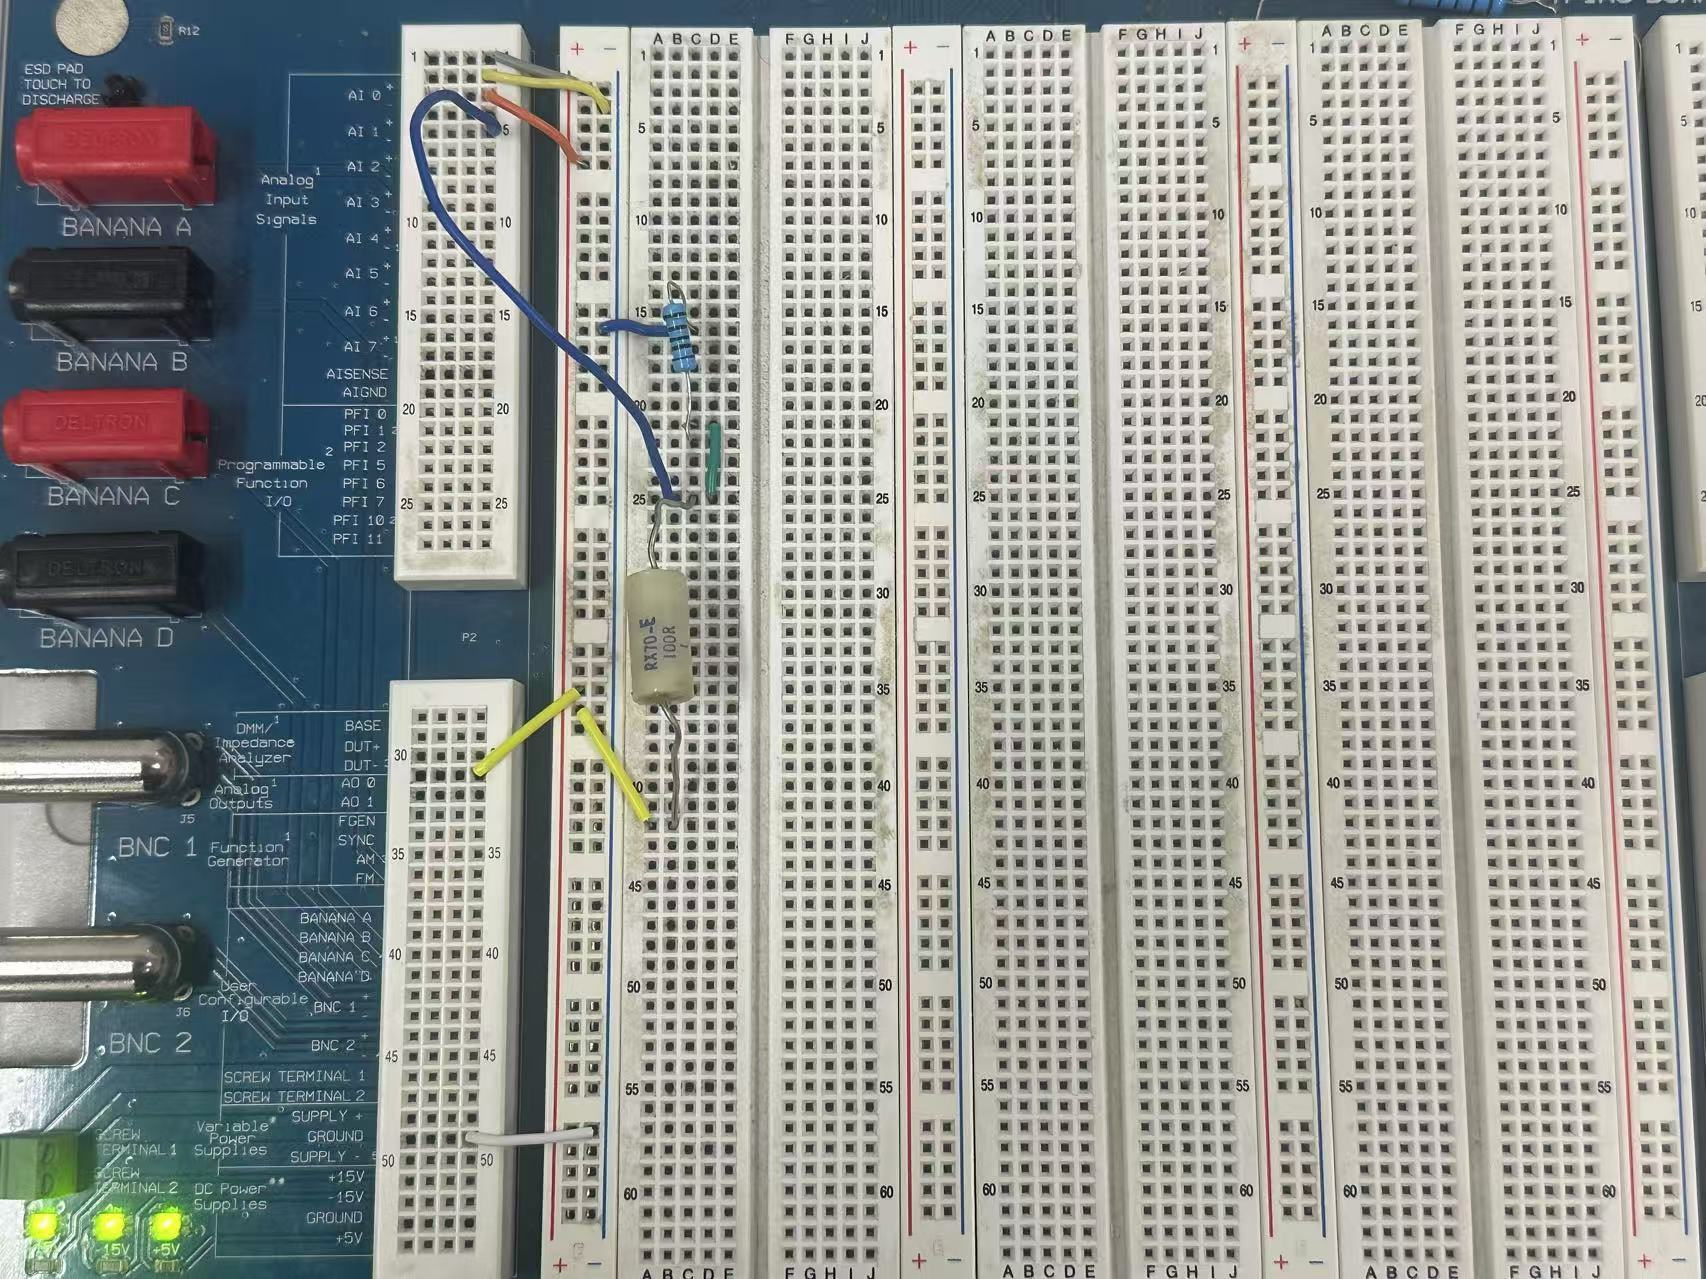
\includegraphics[width=0.6\textwidth]{data/board_circuit.jpg}
    \caption{伏安特性曲线实际电路连接}
    \label{fig:iv_curve_circuit}
\end{figure}

\section{实验数据及处理}
在实验4中, 对50\,$\Omega$ 和 1\,k$\Omega$ 两个电阻进行了测量, 得到的数据如表\ref{tab:exp4_data50}所示.

\begin{table}[H]
    \centering
    \begin{tabular}{|c|c|c|c|c|c|c|c|} 
    \hline
    序号 & 1       & 2      & 3      & 4      & 5      & 6      & 7       \\ 
    \hline
    电压 (\unit{V})& -0.0013 & 0.4505 & 0.9025 & 1.3540 & 1.8060 & 2.2588 & 2.7105  \\ 
    \hline
    电流 (\unit{A})& 0.0000  & 0.0005 & 0.0010 & 0.0014 & 0.0019 & 0.0024 & 0.0029  \\ 
    \hline
    序号 & 8       & 9      & 10     & 11     & 12     & 13     & 14      \\ 
    \hline
    电压 (\unit{V})& 3.1616  & 3.6134 & 4.0655 & 4.5176 & 4.9681 & 5.4198 & 5.8723  \\ 
    \hline
    电流 (\unit{A})& 0.0033  & 0.0038 & 0.0043 & 0.0048 & 0.0052 & 0.0057 & 0.0062  \\ 
    \hline
    序号 & 15      & 16     & 17     & 18     & 19     & 20     & 21      \\ 
    \hline
    电压 (\unit{V})& 6.3253  & 6.7768 & 7.2279 & 7.6801 & 8.1315 & 8.5827 & 9.0352  \\ 
    \hline
    电流 (\unit{A})& 0.0067  & 0.0072 & 0.0076 & 0.0081 & 0.0086 & 0.0091 & 0.0095  \\
    \hline
    \end{tabular}
    \caption{50\,$\Omega$ 电阻的电压-电流数据}
    \label{tab:exp4_data50}
\end{table}

由此数据, 我们可以绘制出50\,$\Omega$ 电阻的伏安特性曲线, 如图\ref{fig:iv_curve_50}所示.

\begin{figure}[H]
    \centering
    
\includegraphics[width=0.7\textwidth]{plot2.pdf}
    \caption{50\,$\Omega$ 电阻的伏安特性曲线}
    \label{fig:iv_curve_50}
\end{figure}

通过最小二乘法拟合, 我们可以得到50\,$\Omega$ 电阻的实际电阻值为$47.95\,\Omega$.

同理, 对1\,k$\Omega$ 电阻进行测量, 得到的数据如表\ref{tab:exp4_data1k}所示.

\begin{table}[H]
\centering
\begin{tabular}{|c|c|c|c|c|c|c|c|} 
\hline
序号 & 1      & 2      & 3      & 4      & 5      & 6      & 7       \\ 
\hline
电压 (\unit{V})& 0.0000 & 0.0148 & 0.0319 & 0.0480 & 0.0641 & 0.0799 & 0.0966  \\ 
\hline
电流 (\unit{A})& 0.0000 & 0.0003 & 0.0007 & 0.0010 & 0.0013 & 0.0017 & 0.0020  \\ 
\hline
序号 & 8      & 9      & 10     & 11     & 12     & 13     & 14      \\ 
\hline
电压 (\unit{V})& 0.1127 & 0.1285 & 0.1449 & 0.1610 & 0.1761 & 0.1925 & 0.2096  \\ 
\hline
电流 (\unit{A})& 0.0023 & 0.0027 & 0.0030 & 0.0033 & 0.0037 & 0.0040 & 0.0044  \\ 
\hline
序号 & 15     & 16     & 17     & 18     & 19     & 20     & 21      \\ 
\hline
电压 (\unit{V})& 0.2254 & 0.2405 & 0.2573 & 0.2747 & 0.2895 & 0.3056 & 0.3213  \\ 
\hline
电流 (\unit{A})& 0.0047 & 0.0050 & 0.0054 & 0.0057 & 0.0060 & 0.0064 & 0.0067  \\
\hline
\end{tabular}
\caption{1\,k$\Omega$ 电阻的电压-电流数据}
\label{tab:exp4_data1k}
\end{table}

通过这些数据, 我们可以绘制出1\,k$\Omega$ 电阻的伏安特性曲线, 如图\ref{fig:iv_curve_1k}所示.

\begin{figure}[H]
    \centering
    
\includegraphics[width=0.7\textwidth]{plot1.pdf}
    \caption{1\,k$\Omega$ 电阻的伏安特性曲线}
    \label{fig:iv_curve_1k}
\end{figure}

通过最小二乘法拟合, 我们可以得到1\,k$\Omega$ 电阻的实际电阻值为$946.16\, \Omega$.

再对二极管进行测量, 得到的数据如表\ref{tab:exp4_data_diode_postive}和表\ref{tab:exp4_data_diode_negative}所示.

\begin{table}[H]
\centering
\begin{tabular}{|c|c|c|c|c|c|c|c|} 
\hline
序号 & 1       & 2      & 3      & 4      & 5      & 6      & 7       \\ 
\hline
电压 (\unit{V})& -0.0016 & 0.0979 & 0.1990 & 0.2978 & 0.3964 & 0.4846 & 0.5474  \\ 
\hline
电流 (\unit{A})& 0.0000  & 0.0000 & 0.0000 & 0.0000 & 0.0000 & 0.0001 & 0.0005  \\ 
\hline
序号 & 8       & 9      & 10     & 11     & 12     & 13     & 14      \\ 
\hline
电压 (\unit{V})& 0.5851  & 0.6108 & 0.6285 & 0.6427 & 0.6530 & 0.6614 & 0.6694  \\ 
\hline
电流 (\unit{A})& 0.0011  & 0.0019 & 0.0027 & 0.0035 & 0.0044 & 0.0053 & 0.0062  \\ 
\hline
序号 & 15      & 16     & 17     & 18     & 19     & 20     & 21      \\ 
\hline
电压 (\unit{V})& 0.6762  & 0.6820 & 0.6868 & 0.6916 & 0.6955 & 0.6978 & 0.6971  \\ 
\hline
电流 (\unit{A})& 0.0072  & 0.0081 & 0.0090 & 0.0100 & 0.0109 & 0.0112 & 0.0111  \\
\hline
\end{tabular}
\caption{二极管正向电压-电流数据}
\label{tab:exp4_data_diode_postive}
\end{table}

\begin{table}[H]
\centering
\begin{tabular}{|c|c|c|c|c|c|c|c|} 
\hline
序号 & 1       & 2      & 3      & 4      & 5      & 6      & 7       \\ 
\hline
电压 (\unit{V})& -0.0016 & 0.0992 & 0.1983 & 0.2985 & 0.3983 & 0.4981 & 0.5986  \\ 
\hline
电流 (\unit{A})& 0.0000  & 0.0000 & 0.0000 & 0.0000 & 0.0000 & 0.0000 & 0.0000  \\ 
\hline
序号 & 8       & 9      & 10     & 11     & 12     & 13     & 14      \\ 
\hline
电压 (\unit{V})& 0.6990  & 0.7979 & 0.8990 & 0.9995 & 1.0983 & 1.1984 & 1.2983  \\ 
\hline
电流 (\unit{A})& 0.0000  & 0.0000 & 0.0000 & 0.0000 & 0.0000 & 0.0000 & 0.0000  \\ 
\hline
序号 & 15      & 16     & 17     & 18     & 19     & 20     & 21      \\ 
\hline
电压 (\unit{V})& 1.3984  & 1.4982 & 1.5987 & 1.6988 & 1.7980 & 1.8991 & 1.9989  \\ 
\hline
电流 (\unit{A})& 0.0000  & 0.0000 & 0.0000 & 0.0000 & 0.0000 & 0.0000 & 0.0000  \\
\hline
\end{tabular}
\caption{二极管反向电压-电流数据}
\label{tab:exp4_data_diode_negative}
\end{table}

通过这些数据, 我们可以绘制出二极管的伏安特性曲线, 如图\ref{fig:iv_curve_diode}所示.

\begin{figure}[H]
    \centering
    
\includegraphics[width=0.7\textwidth]{plot3.pdf}
    \caption{二极管的伏安特性曲线}
    \label{fig:iv_curve_diode}
\end{figure}

\section{实验总结和感想}
本实验主要通过LABVIEW软件, 结合NI ELVIS II+硬件平台, 实现了虚拟仪器的设计与应用. 
通过实验, 我们学会了如何使用LABVIEW软件进行虚拟仪器的设计, 并且实现了对电阻和二极管的伏安特性曲线的测量. 

LabVIEW直观易学, 使用虚拟仪器（VI）和连线来表示程序逻辑，而不是传统的文本代码, 
程序的执行顺序由数据流向决定，符合自然思维方式，更容易理解和调试.
同时, 软件提供大量预定义的 UI 控件、分析函数、仪器驱动等，可以快速构建应用程序，提高开发效率.

但是, 我认为图形化编程也有一些缺点. 
一方面, 当程序逻辑变得复杂时，连线可能会变得混乱，难以维护,
本次的实验4中, 由于需要在循环中进行数据的存储和传递, 连线较为复杂, 使得程序框图变得混乱.
同时, 对于不熟悉 LabVIEW 的人来说，理解图形化的代码可能不如文本代码直观,
具有良好注释的文本代码的表达可能比图形化代码更清晰.
再者, 图形化编程的版本控制也可能不如文本代码方便, 
如果项目的周期较长，或者需要多人协作，无法使用Git之类的版本控制工具进行版本控制.

本次实验的主要难点在于实验4, 它的程序框图相当复杂, 执行逻辑也需要努力理解.
所以在实验中需要认真阅读讲义, 仔细分析实验要求, 以及多次尝试核对参考程序框图
不断修改, 才能顺利完成实验. 我认为想这样复杂的程序使用
文本代码来实现可能会更加清晰简单, 同时我希望LabVIEW也能够提供更多的辅助工具,
如专门用作调试和异常处理的工具, 以提高程序的可读性和可维护性.

\section{思考题}
\textbf{虚拟仪器系统与传统仪器有什么区别，请简要说明}
~\\
传统仪器是硬件定义功能的“专用工具”，其功能固定、显示方式单一，数据处理能力有限，
自动化程度较低，且硬件改动困难，灵活性差。例如，一个传统万用表只能测量电压、电流、电阻等基本参数，
显示方式也仅限于数字或指针，无法进行复杂的分析或数据存储。
而虚拟仪器系统则是一种“软件定义的仪器”，它基于计算机软硬件平台，
利用图形化编程等方式，将仪器功能以软件形式实现。这使得虚拟仪器系统不仅能提供多样化的数据显示方式，
还能进行强大的数据处理和分析，实现高自动化测量，且可以通过软件灵活更改仪器功能，
适应不同的测试需求，并能方便地进行数据传输和网络化管理，
例如在实验中进行线性拟合计算电阻值，或者实现远程操控仪器。
简而言之，虚拟仪器突破了传统仪器的局限性，在灵活性、功能性、智能化等方面都具有显著优势，
代表了仪器仪表的发展方向。

\textbf{本实验内容3中的电压输出和采集哪个先执行}
~\\
先进行电压输出，然后在原型版电路上将电压输入到采集端口，进行电压采集
\end{document}
